\section{Radio Astronomy}\label{ra}
Radio astronomy is the study of inter- and extragalactic objects by collecting and studying the electromagnetic signals they emit. In 1928, a physicist, Karl Guthe Jansky, was searching for possible sources of radio interference for transatlantic communication. What he discovered was a large amount of noise coming from the center of our galaxy and from this the field of radio astronomy was born. Unlike optical telescopes, radio telescopes are able to see through the dust of our galaxy to give us better insight into what lies in its center. Radio frequency radiation is also emitted from cold sources, allowing us to view extragalactic bodies with greater quality and better precision\footnote{Taken from https://public.nrao.edu/radioastronomy/what-is-radio-astronomy}.
%--------------------------------------------------------------------------------------
\subsection{Radio Telescopes}\label{ra:sec:rt}
%
\subsubsection{Radio Telescope Design}
The most common design for radio telescopes is that of the parabolic reflector antenna. The design is a large parabolic dish with a sub-reflector at the parabola's focal point channeling the input into the feed horn at the center of the dish; a diagram of this can be seen in Figure \ref{ra:fig:para}. While it is possible to have a single antenna as a telescope for radio astronomy, in order for them to produce meaningful results, the antennas need to be extremely large (diameter of $+70$ m) which in most cases can be structurally infeasible especially if the antenna is made to be steerable. Instead, a series of smaller ($8\sim30$ m) antenna are used collectively in an array to produce more accurate signal detection. These arrays do so through radio interferometry \citep{cheng2009radio}.
%
\begin{figure}[H]
	\centering
	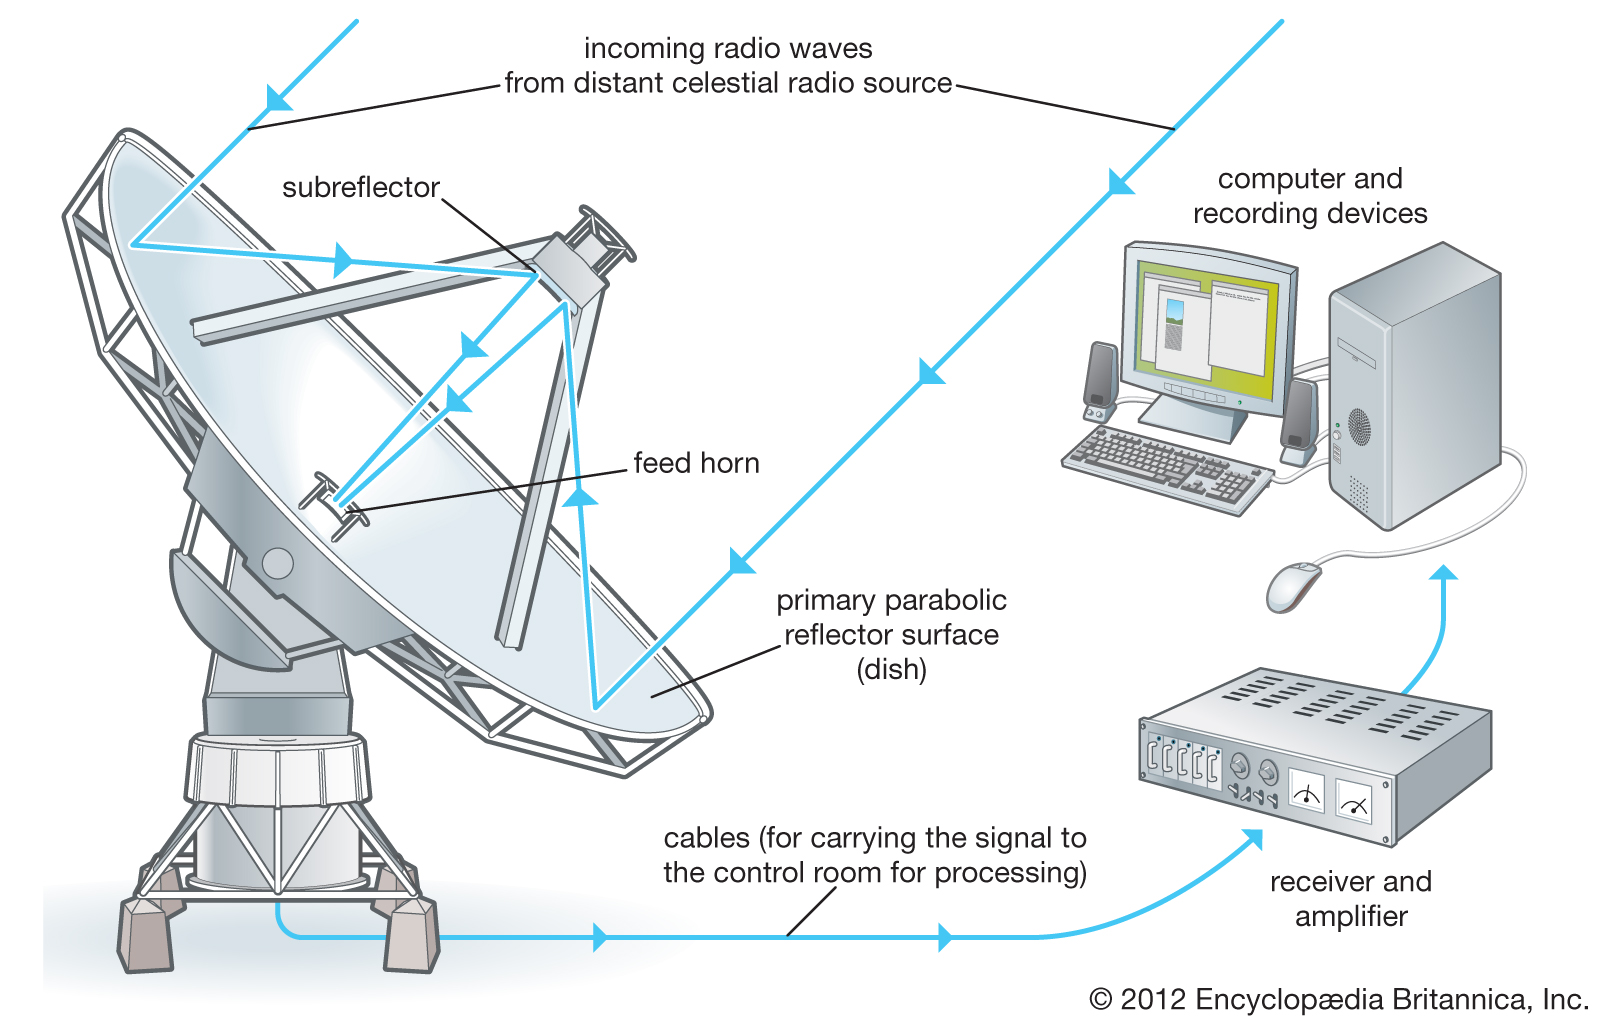
\includegraphics[width=0.5\textwidth]{Images/Telescope.jpg}
	\caption[]{Parabolic reflector antenna design\footnotemark.}
	\label{ra:fig:para}
\end{figure}
\footnotetext{Taken from \url{http://kids.britannica.com/comptons/art-145514}}
%
\subsubsection{Radio Interferometry}\label{ra:ssec:des}
Radio interferometry uses an array of antennas to detect and measure objects emitting radiation in the radio-wave frequencies. Radio waves are defined as electromagnetic radiation with wavelengths of the order of $10^{-3}$ to $10^5$ m \citep{cheng2009radio}. The interferometer finds the source of these waves by detecting correlations in the parallel ray signal transmitted by the radiating source \citet{tasse2016tessellation} and collected by multiple antennas to determine the delay as well as the amplitude and frequency of the source to calculate the position, size and intensity of the source \citep{thompson2008interferometry}.
%
\subsubsection{Radio Telescope Mounts}\label{ra:ssec:mount}
The choice of mount used for a radio telescope plays a large role in how well the telescope is able to track an object. The two main models used are the altazimuth and equatorial mounts. An altazimuth mount rotates on two independent axes, giving it a large range of motion. The equatorial mount has one axis which is fixed to be parallel to the equator. This allows the antenna to simply move across the sky in one direction to track an object. The equatorial mount also follows the natural rotation of the sky as it passes to obtain less distortion (discussed in Section \ref{ra:ssec:eec}) than an altazimuth mount. Altazimuth mounts are still more common as they are relatively cheaper and easier to build than an equatorial mount \citep{thompson2008interferometry}.
%
%\subsubsection{The SKA}
%--------------------------------------------------------------------------------------
\subsection{Image Capturing and Processing}\label{ra:sec:ic}
%
\subsubsection{Aperture Synthesis}\label{ra:ssec:rii}
The electromagnetic radiation collected by the antenna is correlated into voltage differences. The data is collected and stored over some hours and the resulting correlations in the data taken in by each antenna in the telescope are Fourier transformed from the frequency domain to the spatial domain, to give a two dimensional image \citep{sault1994multi}.
%
\subsubsection{The Primary Beam}\label{ra:ssec:tpb}
The primary beam is a mathematical function that describes the sensitivity pattern of an antenna. Naturally the beam is most sensitive in the center of the direction in which the antenna is facing, with fringes of sensitivity radiating out shown in Figure \ref{ra:fig:beam}. The circular sensitivity present in Figure \ref{ra:fig:beam} can be seen affecting the uncorrected image present in Figure \ref{ra:fig:uncorr} \citep{thompson2008interferometry}.
%
\begin{figure}[H]
  \begin{subfigure}{0.45\textwidth}
	\centering
	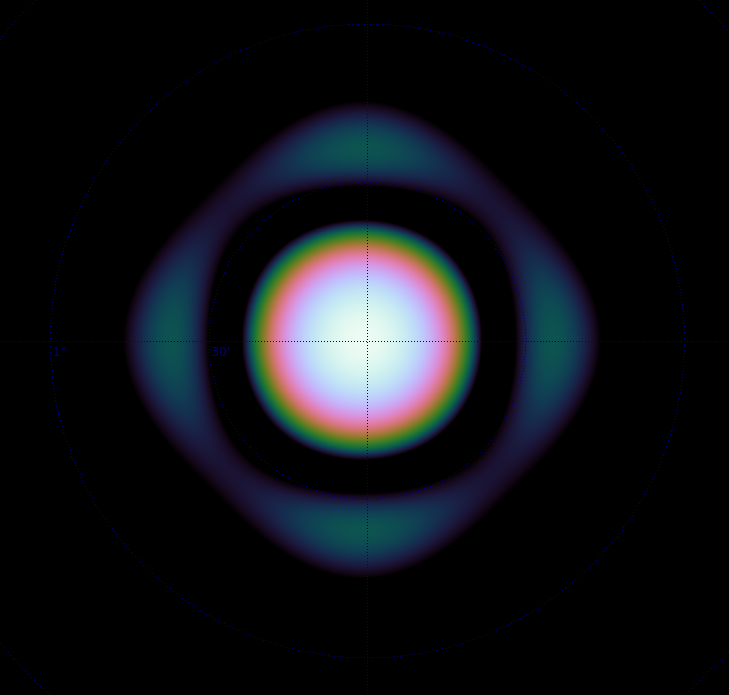
\includegraphics[width=0.9\textwidth]{Images/beam.png}
	\caption{Sensitivity pattern.}
	\label{ra:fig:beam}
  \end{subfigure}
  \begin{subfigure}{0.45\textwidth}
	\centering
	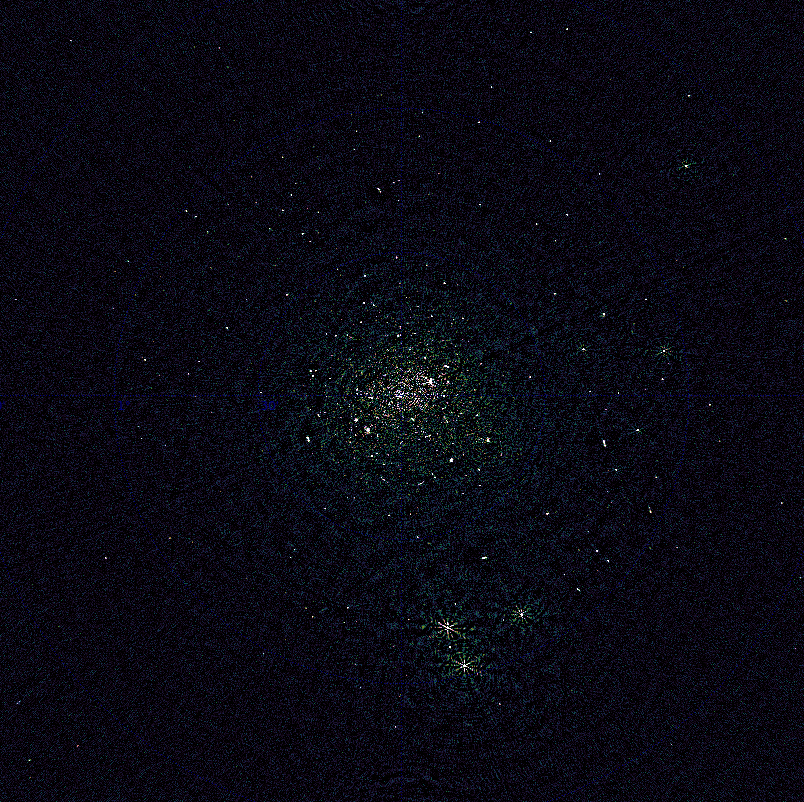
\includegraphics[width=0.9\textwidth]{Images/uncorrected-image.png}
	\caption{Resulting uncorrected image produced through radio interferometry.}
	\label{ra:fig:uncorr}
  \end{subfigure}
  \caption{Primary beam and its effects.}
\end{figure}
%
\subsubsection{Errors and Error Correction}\label{ra:ssec:eec}
As with any real-world data input, the image capturing process of radio interferometry is subject to errors. These errors can be classified as arising from two main groups, namely \gls{di} and \gls{dd} effects \citep{smirnov2011revisiting}. \gls{di} effects are due to differences in the top layer of the atmosphere distorting the signal. This is also known as the complex gain and can be easily corrected for. The \gls{dd} effects in particular arise from distortions due to interference from the ionosphere and deviations of the primary beam from the sky rotation model (due to altazimuth mounts discussed in Section \ref{ra:ssec:mount}). This distortion, $D$, can be corrected, but only relative to a chosen point, $\xi$. The correction at $\xi$ is almost perfect, but as the correction drifts further from $\xi$, it introduces an error which propagates away from $\xi$. This error, $E_i$ at $x_i$ is dependent on the intensity at point $x_i$, $I_i$, and the distortion at the point relative to $\xi$, $D(x_i,\xi)$. Therefore, to minimize this error, every point can be made a correction seed and the image can be broken up according to these points and reassembled to form an image with little to no error. However, this is very computationally intensive as there are hundreds of sources per image and the image is sparely populated. We therefore seek a method that optimises both computational feasibility and error reduction \citep{smirnov2015radio}.
%--------------------------------------------------------------------------------------
\subsection{Naive Method for Error Correction}
The most basic compromise is dividing the image evenly into a grid of smaller images and correcting for these from either the center of the sub-image, the point with the strongest source, or the ``center of mass'' (average location of points) of all the points in the sub-image, either weighted by intensity or not. The problem with this method is that the sub-image is void and has no definite points or if $\xi$ is set at the center, it could be far from every other point and would have no substantial effect on reducing the overall error or if $\xi$ is set at the strongest source or the center of mass, it could lie too close to the boundary of the sub-image and, again, have no overall impact on error reduction \citep{tasse2016tessellation}. An example can be seen in Figure \ref{ra:fig:cor23}.
%
\begin{figure}[H]
	\centering
	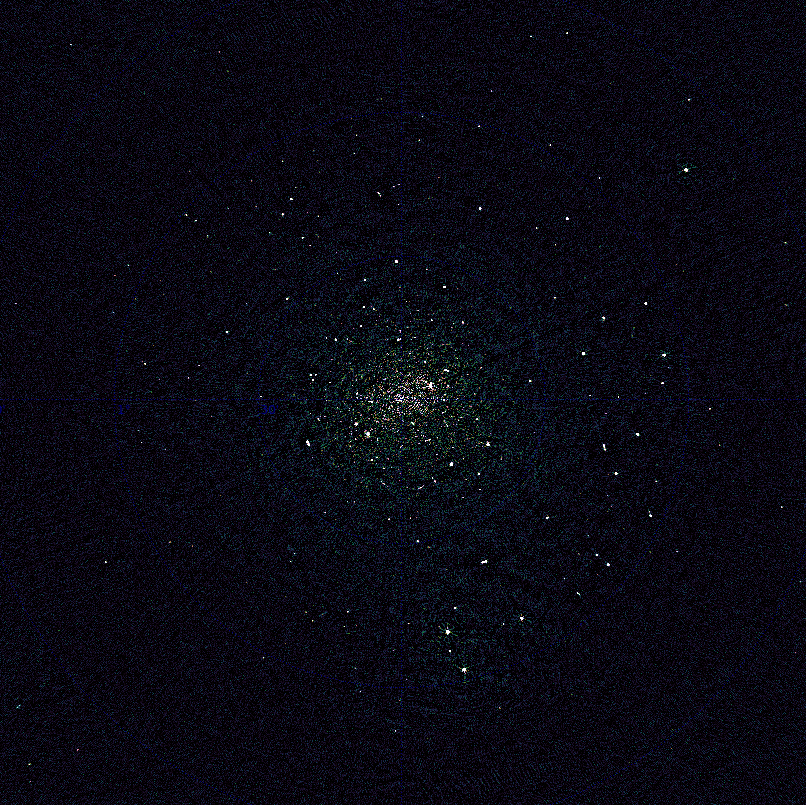
\includegraphics[width=0.5\textwidth]{Images/corrected-23x23.png}
	\caption{Figure \ref{ra:fig:uncorr} corrected on a $23\times23$ grid.}
	\label{ra:fig:cor23}
\end{figure}
%--------------------------------------------------------------------------------------



